\documentclass[jou]{apa} %can be jou (for journal), man (manuscript) or doc (document)
%
%
%these next packages extend the apa class to allow for including statistical and graphic commands
\usepackage{url}   %this allows us to cite URLs in the text
\usepackage{graphicx}  %allows for graphic to float when doing jou or doc style

% 11-07 is the FDG paper.
% 10-08 is robert's thesis.
% APA style info at: http://www.ilsp.gr/homepages/protopapas/apacls.html

% We need a table that shows "Dorm Energy Competition Design", with entries to say if the
% designers revealed (a) how baseline data was collected; (b) how the ranking was
% determined; (c) what factors were taken into account in creating the ranking; (d) was
% data collected after the competition to look for rebound effect; (e) was there evidence
% of short-term, unsustainable behavior change; 

% Proposal: let the teams create an argument for why they should win (this encourages more
% introspection and potentially data gathering.)

\title{Lights Off.  Game On? \\ \ 
       Myths and fixes for energy competition game design}
\author{Philip M. Johnson, Yongwen Xu, Robert S. Brewer, George E. Lee, Michelle Katchuck,
  Carleton A. Moore}
\affiliation{Collaborative Software Development Laboratory \\ Information and Computer
  Sciences \\ University of Hawaii \\ Honolulu, HI USA \\ johnson@hawaii.edu}

\abstract{

  The Kukui Cup project investigates the use of ``meaningful play'' to facilitate energy
  awareness, conservation and behavioral change.  Each Kukui Cup Challenge combines real
  world and online environments in an attempt to combine information technology, game
  mechanics, educational pedagogy, and incentives in a synergistic and engaging
  fashion.  We challenge players to: (1) acquire more sophistication about energy concepts
  and (2) experiment with new behaviors ranging from micro (such as turning off the lights
  or installing a CFL) to macro (such as taking energy-related courses, joining
  environmental groups, and political/social advocacy.)

  To inform the design of the inaugural 2011 Kukui Cup, we relied heavily on prior
  collegiate energy competitions, of which there have been over 150 in the past few years.
  Published accounts of these competitions indicate that they achieve dramatic reductions
  in energy usage (a median of 22\%) and cost savings of tens of thousands of dollars.  In
  our case, the data collected from the 2011 Kukui Cup was generally in agreement, with
  observed energy reductions of up to 16\% when using data collection and analysis
  techniques typical to these competitions.  However, our analysis process caused us to
  look more closely at the methods employed to produce outcome data for energy
  competitions, with unexpected results.

  We now believe that energy competitions make significant unwarranted assumptions about
  the data they collect and the way they analyze it, which calls into question both the
  accuracy of published results from this literature and their effectiveness as serious
  games.  We believe a closer examination of these issues by the community can help
  improve the design not only of future energy challenges, but other similar forms of
  serious games for sustainability.

  In this paper, we describe the Kukui Cup, the design ``myths'' it
  uncovered, and the ``fixes'' we propose to improve future forms of
  ``meaningful play'' with respect to energy in particular and sustainability in general.

}


\acknowledgements{The Kukui Cup is supported in part by grant IIS-1017126 from the
  National Science Foundation, by the University of Hawaii (Facilities Management,
  Housing, and Information and Computer Sciences), by the Hawaii State Department of
  Business, Economic Development, and Tourism, and by the HEI Charitable Foundation.  We
  gratefully acknowledge the 418 players of the 2011 Kukui Cup and the members of the
  project team in addition to the authors who made the vision a reality: Kaveh Abhari,
  Hana Bowers, Greg Burgess, Caterina Desiato, Risa Khamsi, Alex Young, and Chris Zorn.}

\shorttitle{Myths and fixes for energy competition game design}
%\rightheader{Right header}
%\leftheader{Left Header}

\begin{document}
\maketitle 

\section{Introduction}  

The rising cost, increasing scarcity, and environmental impact of fossil fuels as an
energy source makes a transition to cleaner, renewable energy sources an international
imperative. Barriers to this transition include the historical success of electrical
utilities in making energy low-cost, ubiquitous, reliable, and easy to access, thus
enabling widespread ignorance about basic energy principles and trade-offs.  In Hawaii,
the need for transition is especially acute, as our state departs from the norm both with
respect to the price of energy and in reliance on fossil fuels as an energy source.

Moving away from petroleum involves technological, political, and social changes,
requiring citizens to not only think differently, but behave differently with respect to
energy policies, methods of generation, and their own consumption. Unfortunately, there is
no tradition of teaching ``energy'' as a core subject area in the United States, even
though this subject appears to be one of the most important emergent issues of the 21st
century. Anecdotal reports indicate the lack of basic energy literacy at the secondary
school level \cite{Ammons2010}.

%% It would be nice to have more citations and examples regarding the "lack of basic
%% energy literacy."

%% Need more citations throughout the document.

One of the most widespread and successful approaches to raising the profile of energy use
is the collegiate dorm energy competition, which has been held on over 150 campuses in the
past few years \cite{Hodge2010}.  Published reports claim that these competitions are
extremely successful.  Hodge finds median reductions in energy use of 22\% and a maximum
reduction of 80\% in energy use for the competitions she studied. A case study of Elon
University claims that a seven week competition reduced energy consumption by 231,454 kWh
and produced \$2,000 in electricity cost savings per week \cite{Durr2010}.

In an attempt to build upon these promising initial results, we began the Kukui Cup
project in 2010.  Our goal is to expand the scope from a relatively simple ``competition''
where the primary outcome measure is energy consumption in kilowatt-hours (kWh) to a more
elaborate ``challenge'' in which we combine information technology, community-based social
marketing, serious games, incentives, and educational pedagogy to support sustained change
in energy-related behaviors.  In addition to measuring kWh consumption, the Kukui Cup also
implements a point system intended to measure and encourage player involvement with
educational materials, workshops, excursions, social media, and group participation.
Through a series of challenges held in residence halls at the University of Hawaii and
elsewhere, we are attempting to gain deeper insight into how these various factors
contribute to positive behavioral change.

Our first Kukui Cup challenge was held at the University of Hawaii in Fall, 2011 for the
1,000 students living in the Hale Aloha residence halls. The challenge divided the
students into 20 teams (called ``lounges'') of approximately 50 students each.  We started
measuring energy consumption for most teams at five weeks prior to the competition,
although several teams did not have operational energy meters until shortly before the
competition started. We followed the traditional approach of using this pre-challenge data
to produce baselines as a way of assessing whether and to what extent energy reductions
occurred as a result of the challenge.

Our initial analyses of the data we collected during the challenge appeared promising.
Over 400 of the students participated in the three week challenge, spending over 850 hours
in the online environment.  Student feedback regarding both real world and online aspects
of the challenge was uniformly positive.  Several teams appeared to achieve a 10-16\%
reduction in their energy usage during the challenge.  Participating students made over
1,000 commitments and earned over 80,000 points.

As we continued to look at the outcomes from the 2011 challenge in order to understand how
to better support sustainable behavioral change, we began to be troubled by the way the
Kukui Cup and other dorm energy competitions measure outcomes, and the variety of
unwarranted assumptions underlying the measurements and results.  These design problems
are not merely theoretical or scientific: they have a direct impact on the experience of
participants and the effectiveness of these competitions as ``meaningful play.''  For
example, the baseline calculation method used during the 2010 Campus Conservation
Nationals energy competition led some students at Oberlin College to stop participating in
the competition ``out of frustration'' \cite{Willens2010}.

Making matters worse, published reports concerning energy competitions rarely document
how, for example, baseline energy consumption is calculated, or the extent to which energy
reductions are sustained after the competition ends.  Without this information, it is
hard to assess the true ``meaningfulness'' of the ``play.''  For example, if incorrectly
defined baselines enable a team to ``coast to victory'' with minimal behavior change,
then is the play ``fair?'' If team energy consumption returns immediately to pre-competition
levels, no matter what level of reduction is achieved during the competition, then is the play ``meaningful?''

This paper presents our findings to date about how to better understand the impact of
energy competitions and challenges as meaningful play, and how to improve this impact over
time.  We believe this process must start with a better understanding of the limitations
of {\em kWh consumed} as an outcome measure, as tempting a metric as it might be.  We
argue that ``behavior'' must be interpreted and measured more broadly and that games must
be designed to promote and reward a much more diverse spectrum of behavior change.  Rather
than reward students for unsustainable, temporary behavior changes such as unplugging
vending machines (as at Oberlin College \cite{Petersen07a}) or camping outside during the
competition (as at Carleton College \cite{Hodge2010}), future games should reward students
for more sustainable, lasting changes such as enrolling in a class on energy in an upcoming
semester, or joining an environmental group that promotes renewable energy.

The next section of this paper provides a brief overview of the Kukui Cup.  The following
section presents the myths (unwarranted assumptions) that we believe to be widespread in the
current design and reporting of energy competitions. We conclude with our fixes (recommendations)
for how we and others should design future energy challenges to be more effective as
meaningful play.

\section{The Kukui Cup}

A defining feature of Kukui Cup challenges is a blend of real world and online
activities, all utilizing game mechanics.  In the real world, players participate in
workshops and excursions, win prizes, and most importantly, learn about their current
lifestyle and its impact on energy consumption.  In the online world of the Kukui Cup web
application, players earn points, achieve badges, increase their sustainability ``literacy''
through readings and videos, and use social networking mechanisms to engage with friends
and family about the issues raised. The challenge is designed to make real world and
online activities complementary and synergistic.

%%  Have a paragraph that says how Makahiki and Kukui Cup were influenced by the following
%%  previous competitions with citations. 

Figure \ref{fig:kukuicup-home-page} illustrates the home page of the web application. 

\begin{figure*}[htbp]
\begin{center}
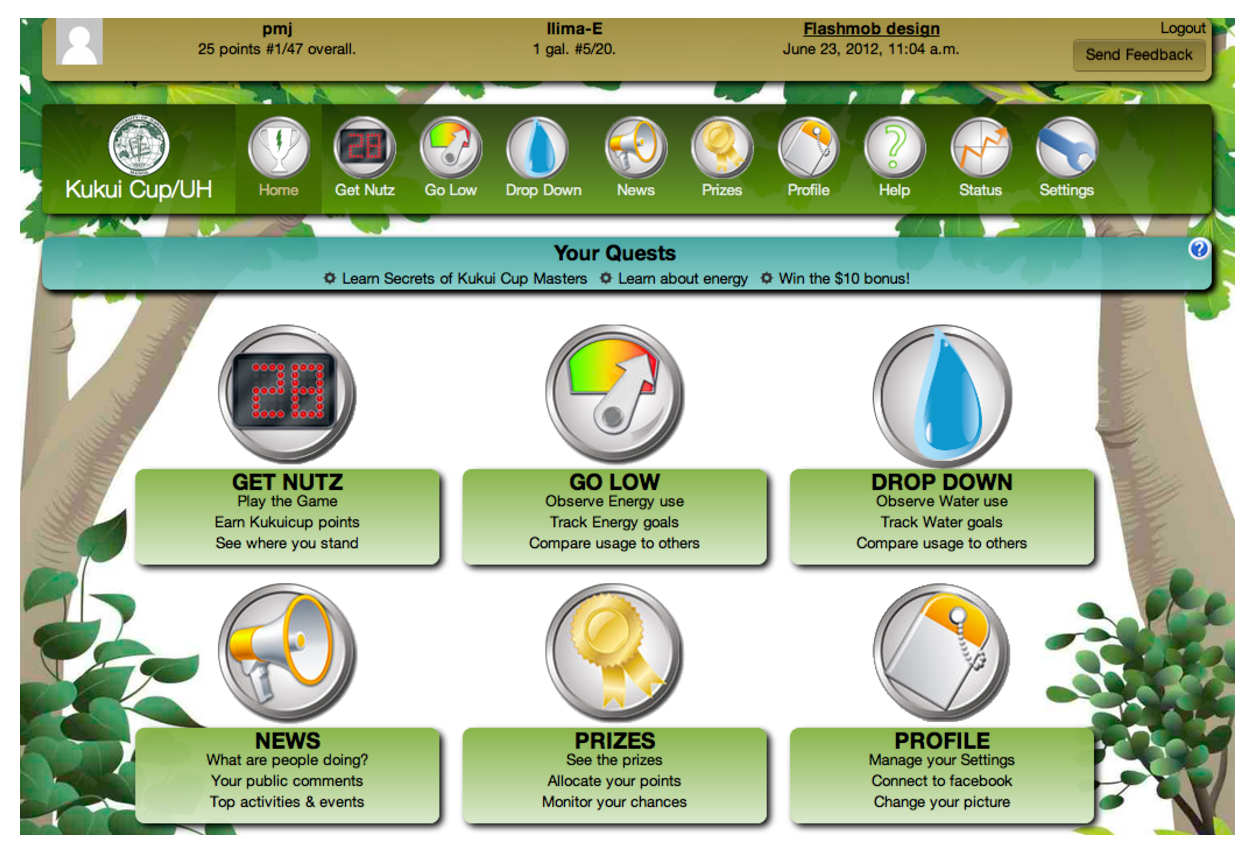
\includegraphics[width=0.8\textwidth]{kc-homepage.eps}
\caption{An example Kukui Cup home page}
\label{fig:kukuicup-home-page}
\end{center}
\end{figure*}


Each Kukui Cup Challenge is typically designed with the following goals for its participants:
\begin{itemize}
\item Increase {\bf knowledge} about energy issues;
\item Gain {\bf insight} about the impact of one's current behaviors.
\item {\bf Motivate} them to change their behaviors for the better;
\item Build {\bf community}, through awareness of local and national sustainability organizations and initiatives;
\item Create {\bf commitment}, from minor (turn off the lights when not in use) to major (pursue a profession related to sustainability).
\end{itemize}

To create sophisticated games based upon energy consumption, it is helpful to integrate
real-time energy data from meters into the challenge through goal tracking and energy
visualizations. We developed WattDepot \cite{csdl2-10-05} to provide an open
source, vendor-neutral framework for energy data collection, storage, analysis, and
visualization.  WattDepot is useful not only as technology infrastructure for the Kukui
Cup, but as infrastructure for other energy-related initiatives such as the Smart Grid.

Implementation of game mechanics is provided by another system we developed called
Makahiki \cite{csdl2-11-07}.  It provides an open source, component-based, extensible
environment for developing sustainability challenges such as the Kukui Cup and tailoring
them to the needs of different organizations.  One configures the Makahiki framework to
produce a ``challenge instance'' with a specific set of game mechanics, user interface
features, and experimental goals.  Makahiki provides sophisticated instrumentation to
support evaluation of how well the game mechanics supported the organization's goals for
the challenge.

\section{Myths and misperceptions in energy challenge game design}

The preceding sections present the design and implementation of the 2011 Kukui Cup along
with some basic outcome data in a manner consistent with the way many other energy
competitions have been presented.  Perhaps the most significant outcome from the 2011
Kukui Cup is the insight that virtually all energy challenges, when viewed as game
designs, contain significant flaws including one or more of the following: (1) they do not
create a fair game, (2) they do not measure what they think they are measuring, (3) they do not
measure the right things, and (4) they do not promote the right outcomes.  In this section we
discuss how we came to these realizations.

To begin: a fundamental property of energy challenges is competition, and a fundamental
property of competitions is the ability to creating rankings.  The first myth involves the
assumption that the traditional ranking method produces valid (i.e. fair) energy competitions.

\subsection{Myth \#1: Percentage reduction from baseline is a fair ranking method}

There are two traditional methods for creating rankings in energy
competitions: (1) by total energy consumption or (2) by reduction from a baseline.

The first ranking method is simple: order the teams according to their total energy
consumption (from least to most) during the competition interval.  As illustrated in Table
\ref{table:total-reduction}, if Team A consumes 1,140 kWh during the competition period,
and Team B consumes 1,239 kWh, then Team A wins.  This is the simplest method, but
produces a fair ranking only if every team is equivalent with respect to the factors
affecting their energy consumption.  For example, to use this ranking method, every team
should have the same number of members.  If Team A has 50 members and Team B has 60
members, then Team A's victory might be due to its unfair advantage of having fewer energy
consumers.  In addition, to use total energy consumption as the ranking method, every team
should have the same energy infrastructure.  If, for example, Team A lives in a
well-insulated building and Team B lives in a poorly insulated building, then Team A again
has an unfair advantage.  Because it is so difficult to obtain equality among teams with
respect to all significant energy consumption factors, and because the unfairness of a
competition using this ranking method can be so obvious, the use of total energy
consumption is relatively uncommon.

\begin{table}[tbp]
\caption{Total energy consumption ranking method. Winning number in bold.}
\label{table:total-reduction}
\begin{tabular}{p{0.5in}p{0.5in}}\thickline
Team  & Actual (kWh) \\ \hline
A     & {\bf 1,140}        \\  
B     & 1,239        \\ \hline
\end{tabular}
\end{table}


In an attempt to address the fairness problems that arise with the total energy
consumption ranking method, the more common approach used by almost all energy
competitions is to compute a ``baseline'' for each team based upon historical usage and
then produce rankings based upon reductions from this baseline.  The hope is to
effectively normalize energy consumption so that teams with differing factors affecting
their energy consumption can be fairly ranked. Table \ref{table:percentage-reduction}
illustrates this approach.

\begin{table}[tbp]
\caption{Reduction from baseline ranking method. Winning numbers in bold.}
\label{table:percentage-reduction}
\begin{tabular}{p{0.5in}p{0.5in}p{0.5in}p{0.5in}p{0.5in}}\thickline
Team  & Baseline (kWh) & Actual (kWh) & Reduction (kWh) & Percent Reduction  \\ \hline
A     & 1,200          & 1,140        & 60                 & {\bf 5 \%}              \\  
B     & 1,300          & 1,239        & {\bf 61}                 & 4.6 \%            \\ \hline
\end{tabular}
\end{table}

As in the prior example, Team A consumes 1,140 kWh and Team B consumes 1,239 kWh.  Using
energy data collected prior to the competition, a baseline of 1,200 kWh is calculated
for Team A and a baseline of 1,300 kWh is calculated for Team B.  

What is interesting about this example is that there are two winning numbers. Team A wins
if {\em percentage reduction} from baseline is used as the ranking method, while Team B wins if
{\em absolute reduction} from baseline is used as the ranking method.  In all of the energy
competitions we have seen, it is percentage reduction from baseline, not absolute
reduction from baseline, that is used as the ranking method.

The uniform use of percentage reduction from baseline as the ranking method reveals one
problem with the use of baselines, because there is no {\em a priori} reason that
percentage reduction from the baseline produces a more fair ranking than absolute
reduction from the baseline.  To see why this is so, consider a (very plausible) scenario where
Team A lives on one floor and Team B lives on an adjacent floor.  The two floors are
similar in structure and occupancy except that Team B's floor includes a shared laundry
room.  In this case, the most fair way to produce a ranking is to calculate the energy
consumption of the shared laundry room, subtract that consumption from Team B's data, then
use absolute values to rank the floors.  Put simply, the two teams should be considered
equal once the load from the shared laundry room is factored out.

\begin{table}[tbp]
\caption{Adjusted absolute consumption ranking method. Winning numbers in bold.}
\label{table:adjusted-absolute-reduction}
\begin{tabular}{p{0.5in}p{0.5in}p{0.5in}p{0.5in}p{0.5in}}\thickline
Team  & Baseline (kWh) & Actual (kWh) & Adjusted Actual (kWh) & Percent Reduction  \\ \hline
A     & 1,000          & 900          & 900            & {\bf 10 \%}        \\  
B     & 1,300          & 1,180        & {\bf 880}      & 9 \%               \\ \hline
\end{tabular}
\end{table}

Table \ref{table:adjusted-absolute-reduction} illustrates this scenario.  Team A reduces
their consumption by 100 kWh from the baseline, for a winning percentage reduction of 10\%. Team B
reduces their consumption by 120 kWh from the baseline, for losing percentage reduction of
9\%.  But the fairer way to compare these two teams is to simply subtract out the 300 kWh
of energy consumed by the laundry room, then compare the two consumptions directly.  Under
this ``adjusted'' ranking scheme, Team B wins because their adjusted actual consumption of 880
kWh is less than Team A's actual consumption of 900 kWh.

Of course, the adjusted absolute consumption ranking method is not a panacea for all
energy competition situations.  If Team A has 50 players and Team B has 70 players, then
some sort of percentage-based normalization to create a ``per capita'' consumption is
required to provide a fair ranking.  In many cases, some combination of absolute
adjustment (to compensate for structural differences like laundry rooms) and
percentage-based adjustment (to compensate for differences in number of players) might be
required to produce a fair ranking.

Our conclusion is the following: to produce a fair ranking based upon 
historical energy consumption, you must determine the reasons behind the differences in
consumption by teams, because those reasons are crucial to creating a fair ranking.

\subsection{Myth \#2: Representative energy data can be collected immediately prior to the competition}

The preceding section assumes that representative, or ``normal'' energy usage during the
competition can be determined from historical data, and then discusses the problems that
arise in using such data to create a fair ranking.  Let's now step back and consider the
question: is it possible to gather historical energy data immediately prior to the
competition and be confident that it reflects representative use (i.e. normal use, as
would occur in the absence of the competition). 

This question is important because many energy competitions create baselines using the
average energy consumption from several weeks immediately prior to the start of
competition.  Using this recent data (as opposed to data from a year or more in the past)
has two significant advantages with respect to obtaining representative data. First, this
data is collected from the players who will actually participate in the competition.
Second, this data is based upon the state of the infrastructure (buildings, appliances,
etc.) as it will be during the competition.

We discovered the problem with this approach after collecting and evaluating energy data
from immediately before the 2011 Kukui Cup. Figure
\ref{fig:kukuicup-baseline-data-chart} shows data from the weeks prior to the
Kukui Cup 2011 energy challenge for five of the 20 teams.

\begin{figure*}[htbp]
\begin{center}
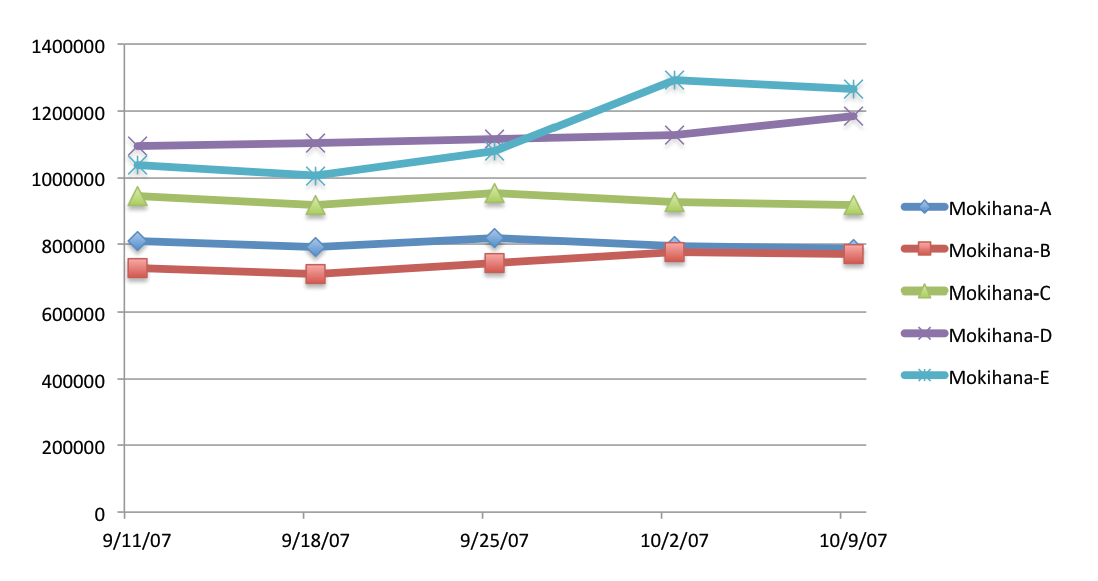
\includegraphics[width=0.8\textwidth]{kc-baselines.2.eps}
\caption{Energy data for five teams for the weeks immediately preceding the 2011 Kukui Cup}
\label{fig:kukuicup-baseline-data-chart}
\end{center}
\end{figure*}

% Would be better for Y axis to be in kWh and Y axis scale from 600 kWh to 1300 kWh (so
% variations are more visually apparent).  

What makes this data problematic for predicting ``normal'' conditions during the
competition are the variety of trends that can be observed in the different teams.  The
energy consumption of Mokihana-A, Mokihana-B, and Mokihana-D is trending upwards, while
the energy consumption of Mokihana-C and Mokihana-E is trending downwards.  The change can
be substantial: in the case of Mokihana-A, weekly energy consumption varies by
approximately 30\% during the five weeks prior to the start of the challenge.

If we are to use this data to predict ``normal'' conditions during the challenge, we must
decide whether the trends represent persistent or transitory changes in consumption.  If
we assume the trends represent persistent changes, then the most representative data is
that collected immediately prior to the start of the challenge.  For example, given this
assumption, Mokihana-E would compete based upon a baseline consumption of approximately 1300
kWh per week.

If, on the other hand, we assume the trends represent transitory changes in consumption,
then a better choice is to compute the baseline from the average energy usage over several
weeks prior to the competition.  Under this assumption, Mokihana-E would compete based
upon a baseline consumption of approximately 1100 kWh.  Thus, the choice between
persistent and transitory assumptions can make a difference of 15-20\% in the baseline value
in real world conditions.

All energy competitions that we have seen that have actually published their baseline
calculation approach use the averaging method, which implicitly assumes that observed
trends are transitory, not persistent.  But there is no {\em a priori} reason to assume
that trends are transitory.  For example, perhaps a half dozen additional residents moved
in to Mokihana-E in late September, creating a persistent increase in energy consumption.
In this case, using the average of several weeks to compute the baseline unfairly
penalizes Mokihana-E by producing a low baseline value that will not reflect ``normal''
conditions during October.  Similarly, using the average approach when consumption is
trending down in a persistent manner (as might be the case if residents move out or
structural improvements are introduced) gives that team an unfair advantage, as their
baseline will be abnormally high.

This same problem can occur when seasonal change is taken into account: the amount of
energy required to heat a team's residence might be significantly less in the month
preceding the competition if the competition is held in the Fall. Similarly,
heating-related energy consumption might be significantly more in the weeks preceding the
competition if the competition is held in the Spring.  

This problem of assuming data collected immediately prior to the competition is
representative caused a significant problem with the first Campus Conservation
Nationals event \cite{Willens2010}.  According to John Peterson, the ``baseline
period... was, in some cases, resulting in percentage changes for individual
buildings... that were more attributable to changes in weather and other factors than to
the choices that students were making in their dorms.''

Our conclusion is the following: Use of data collected immediately prior to the
competition can predict ``normal'' conditions during the competition with limited
accuracy. Depending upon the choice of assumptions, baseline values can vary by at least
20\% under real world conditions.  This issue alone is enough to wipe out (or create) the median
energy reductions found in published energy competition results.

\subsection{Myth \#3: Representative energy data can be collected from years  prior to the competition.}

Given the problems with obtaining representative data immediately prior to the competition
for the purpose of creating baselines, an alternative is to use data from prior years.
This was in fact the choice made during the first Campus Conservation Nationals event
\cite{Willens2010}, as it was felt that such data would take into account seasonal changes
more effectively than data collected immediately prior to the competition. Unfortunately,
using data from prior years has significant validity problems when used to represent
``normal'' energy consumption during a future year, including:

\begin{itemize}

\item The residents of the building are typically different from year to year.
  Individuals can vary significantly in their energy consumption, and there is no {\em a
    priori} reason to believe that these differences simply average out. 

\item Building infrastructure can change from year to year. HVAC and other energy systems
  can degrade (leading to more energy consumption in future years) or be updated (leading
  to significantly less energy consumption in future years).  Similarly, building
  maintenance (such as weather stripping, lighting upgrades, etc.) can all change the
  energy consumption needs significantly.

\item Weather can vary considerably from year to year.  The number of heating degree days and cooling
  degree days in a given month can change considerably from one year to the next, leading
  to volatility in energy demand. 

\end{itemize}

As one example, we examined the energy consumption data for the month of October for the
past 12 years in the Hale Aloha residence halls, and discovered variability of over 30\%
from one year to the next. In Hawaii, this variability cannot be attributed to seasonal
variation (the Hale Aloha residence halls have neither centralized heating nor cooling)
but due to some combination of changes in the energy habits of the residents and ongoing
building infrastructure changes.

As another example, consider the outcome data graphic regarding the 2011 Green Cup at University of
California, Berkeley \cite{Dhong2011}, shown in Figure \ref{fig:ucb-green-cup}.

\begin{figure*}[htbp]
\begin{center}
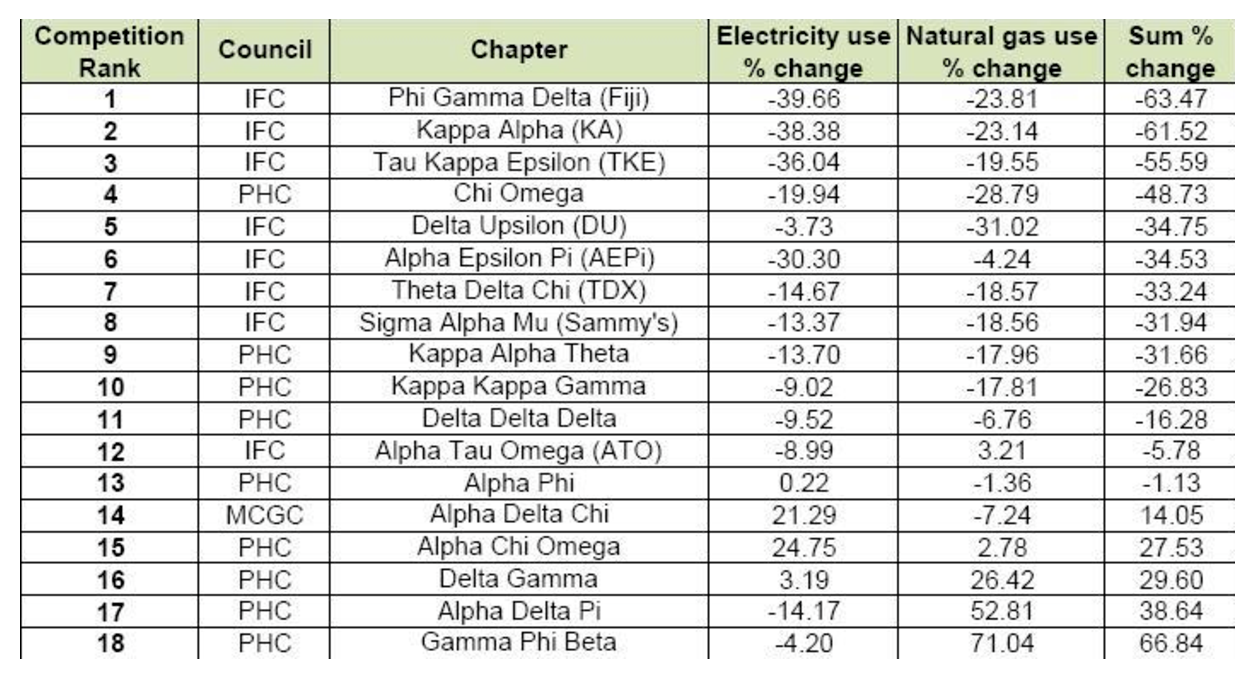
\includegraphics[width=0.8\textwidth]{ucb-green-cup.png.eps}
\caption{Outcome data for the 2011 UC Berkeley Green Cup}
\label{fig:ucb-green-cup}
\end{center}
\end{figure*}

This table shows the reported changes in both electricity and natural gas consumption for
18 fraternity houses during a two month competition.  The houses ``are ranked based upon
reductions in per-capita electricity and natural gas relative to individual chapter
baselines''.  The baselines were based on the ``house's previous energy bills for the same
two months.''  

What this report fails to discuss is the huge amount of variation in results among
houses. With respect to electricity consumption, results varied from -39\% to +24\%.  With
respect to natural gas consumption, results varied from -31\% to +71\%.  The aggregate
outcome measure (sum of percentage change in both electricity and gas) varies a staggering
amount: from -63\% to +66\%.  

What is the cause of this extreme variability in results?  One possibility is that the behaviors
of the occupants of houses changed in wildly different manners in response to the
competition, with some houses deciding to conserve, and others deciding to increase
their consumption.  This explanation seems quite implausible.  An alternative, more plausible
explanation is that their use of baseline data from prior years was not a valid predictor of
the ``normal'' consumption to be expected in the absence of the competition. If so, one
cannot say with any confidence who won and how much was saved. 

Our conclusion is the following: Similar to data collected immediately prior to a
competition, data collected from prior years can predict ``normal'' conditions during the
competition with only limited accuracy.  The Kukui Cup data suggests that the margin of error can easily
exceed 20\%.  The Green Cup data suggests that the margin of error could be even greater. 


\subsection{Myth \#4: Competition data can be used to estimate actual savings}

Most energy competitions report on the cost savings generated due to changed behaviors.
For example, the Campus Conservation Nationals reported that ``savings nationwide totaled 509,000
kilowatt hours, \$50,200, and 816,00 pounds of carbon dioxide'' \cite{Willens2010}.  The UC
Berkeley Green Cup report states that ``29,221.17 kWh of electricity and 667.33 Therms of
natural gas were saved'' \cite{Dhong2011}.

Unfortunately, our analysis calls into question the assumption underlying these claims,
that it is possible to gather energy data that can serve as ``representative'' of the
consumption to be expected during the competition. 

Unfortunately, if it is not possible to generate representative consumption with any
accuracy, then it is not possible to estimate actual savings with any accuracy.  This is
because estimated savings are always calculated by assuming that the baseline data not
only puts teams on an equal footing with each other for the purposes of the competition,
but also represents an accurate prediction of what each team would have consumed during
the time interval of the competition, had the competition not taken place.  

It is interesting to note that these two applications of baseline data are
independent: it is plausible to design baselines that succeed in creating a
level playing field among teams but that do not predict what the energy
consumption would have been in the absence of the competition.

Our conclusion is the following: virtually all published claims for dollar savings due to
energy competitions could not withstand a detailed analysis of the assumptions upon which
these claims were made.  

\subsection{Myth \#5: The ``good guys'' win}

One intuitive assumption concerning energy competitions is that the winners will be those
who are most energy conscious.  In reality, under typical competition conditions
(i.e. collection of baseline data immediately prior to the competition, and the use of
percentage reduction from baseline for ranking), those teams who are most energy conscious
prior to the competition might be at a distinct disadvantage.

This is because energy conscious teams are more likely to have already been practicing 
conservation oriented behaviors prior to the competition period, and thus
their baseline energy use will be lower than their ``energy hog'' peers.  This makes it
harder for them to compete on the basis of percentage reduction, since they have less
``fat'' (from an energy perspective) to cut from their consumption.  As a concrete example, we
discovered that it is not uncommon for residence hall rooms to have two refrigerators and
a few even had three refrigerators. For those residents, simply turning off one
refrigerator for the duration of the competition can achieve significant reductions in
consumption, whereas more ecologically conscious residents who chose to use only one
refrigerator would have to forego the refrigerator entirely to obtain the same reduction.

Our conclusion is the following: although the good guys do not necessarily win, this is
not necessarily a bad thing. It is possible that giving positive reinforcement to
profligate energy users might be more effective than rewarding those who have already
bought into energy conservation principles. What is missing is an understanding of whether
this phenomenon is occurring and what the effectiveness of rewarding this group actually is.


\subsection{Myth \#6: Competitions encourage sustainable behavior change}

% Can we simply say "there are N reports of dorm energy competitions"?

It is an implicit assumption of all collegiate energy competitions that students will acquire
sustainable, energy conscious behaviors as a result of participation.  If this was not so,
if the goal was only to reduce energy consumption during the competition period, then far
easier approaches could be implemented (for example, rolling blackouts.)

What is remarkable about published reports of energy competitions is the lack of evidence
for sustained, positive behavior change. Instead, reports indicate unsustainable changes,
from unplugging vending machines \cite{Petersen07a} to camping outside \cite{Hodge2010} to 
{\em (cite other unsustainable behaviors here)}.   With few exceptions, reports do not
track or analyze anything about what happens after the competition ends, even though this
is perhaps the most important behavioral question of all.  

Our conclusion: We believe this absence of post-competition information is mostly due to
the student-run nature of collegiate energy challenges, where all time and energy is
focused on the event itself, and once the event is over, there appears to be nothing more
to be done. To fix this, student organizers must become aware of the importance of
post-competition monitoring and assessment and allocate their time and resources
accordingly.

\subsection{Myth \#7: Energy competitions measure the right thing}

We believe that measuring {\em percentage change from baseline} is so widespread because
it appears to have so many appealing properties.  First, measuring in-competition energy
consumption energy use is extremely easy, as is the collection of pre-competition data.
Second, using percentage change from baseline as a ranking method appears more valid than
ranking according to absolute energy use. Third, it is straightforward to convert reduction
values into ``dollars saved'' by multiplying by the local cost per kilowatt-hour.

The fact that this approach is easy does not make it appropriate for at least two
reasons.  First, as the preceding myths have discussed in detail, there is considerable
evidence that the numbers produced are not accurate: baseline data as collected for energy
competitions do not appear to be valid as predictors of ``normal'' consumption in the absence
of the competition during the time intervals of interest.  

Second, measuring and reporting only consumption data during the competition misses the
most meaningful data of all: the behaviors and energy consumption that occurs after the
competition is over. For example, if consumption simply returns to its precompetition
level, then the impact of the competition is unclear. Furthermore, it incentivizes
unsustainable, short-term, radical changes in behaviors which students undertake only
because they know they can cease to follow them within a short period of time.

Our conclusion: the almost exclusive focus of collegiate energy competitions on measuring
percentage reduction from baseline during the competition leads to (1) invalid claims
regarding savings and (2) an incentive to engage in unsustainable behaviors.

\section{Supporting more meaningful play through improved energy challenge game design}

We claim that the effectiveness of energy competitions can be improved if they provide
better opportunities for both meaning (in the sense of sophisticated insight as well as
impact upon future behavior) and play (in the sense of providing fair competitions as well
as providing other, non-competitive forms of play). We conclude with our recommendations
for game design ``fixes'' resulting from our experiences with the 2011 Kukui Cup and
analysis of other energy competitions.

\subsection{Fix \#1: Don't compete on kWh}

Perhaps the single most important fix for future energy challenge game design is to
abandon {\em kWh consumed} as the primary outcome measure.  As an example of an 
alternative, the Kukui Cup implements a competition in which players and teams compete
based upon a point system, where points can be earned for successfully answering questions
about energy videos, attending workshops and excursions, and other sustainability-related
activities.  The 2011 Kukui Cup also had a competition based upon kWh consumed, but
because the infrastructure for the Hale Aloha residence hall floors is so similar, we
measured absolute energy consumption rather than a percentage reduction from baseline.

Avoiding competitions based upon kWh consumed helps to address at least the first four myths.

While we advocate against competition based upon kWh, this does not imply that measurement
of consumption has no use.  In fact, measurements of kWh consumed still have a very important role:
as empirical feedback to help players understand and assess the impact of structural and
behavioral change.

\subsection{Fix \#2: Use long time intervals}

Hodge states that one of the five core components of collegiate energy competitions is
``a short timeframe'', and that this ``can be a catalyst for students to go all out, which
in turn creates hype and energy'' \cite{Hodge2010}.   Based upon our analyses, we believe
that a short time frame encourages exactly the wrong behaviors:  short-term, unsustainable
changes that the players have no intention of retaining after the competition ends.  

Instead, we recommend that future energy challenge games last a minimum of four months:
too long a time for students to camp outside, unplug their vending machines, and so forth.
By analogy, the strategies for winning an energy ``marathon'' are very different, and much
more likely to be sustainable than the strategies for winning a ``sprint''.

We believe this fix helps to address Myth \#6.

\subsection{Fix \#3: Use dynamic baselines}

As discussed in depth above, we believe that current approaches to baseline computation
are, in most cases, irreparably flawed.  Yet providing an objective measure of progress is
very useful to creating effective meaningful play.  

We claim that the problem with current approaches to baselines is that they are used to
both measure ``progress'' with respect to behavior change as well as an estimate of what
``normal'' consumption would have been in the absence of the challenge.

We recommend that future energy challenges address these two issues independently.  For
example, an alternative type of baseline that can be used to measure progress is one based
upon a ``sliding window'' of average consumption for each team over the preceding few
weeks, and the goal is to simply stay under this ``baseline of the recent past'', where
the recent past can and will include at least a portion of the competition interval itself.

The use of a sliding window means that the baseline is no longer static, but rather
changes throughout the competition, and thus incentivizes sustainable changes (because each
reduction in consumption is incorporated into the baseline measurement and thus impacts on 
the goal behavior.)  This aspect helps to address Myth \#6. 

The second impact of a sliding baseline is its obvious inapplicability as an estimator for
normal consumption in the absence of the challenge.  This aspect helps to address Myth \#4.


\subsection{Fix \#4: Measure both micro and macro behavioral change}

Traditional energy competitions tend to focus on what we call ``micro'' behavioral
changes, such as turning off the lights when you leave the room, enabling the screen saver
on your computer, and so forth.  These are meaningful changes, but there exists another
level that we call ``macro'' behavioral change.  Examples of macro behavioral change
include: choosing to put off buying a car until a hybrid or EV can be obtained; choosing
to enroll in a course on sustainability or energy issues; choosing a degree program
related to energy or sustainability; choosing political candidates to vote for based (in
part) on their energy views; and choosing a job (during or after school) based upon the
work's impact on energy or sustainability.  Micro behaviors tend to involve habits, while
macro behaviors tend to involve decision making.

Considering macro behavioral change precipitates a significant shift in thinking about
almost every aspect of an energy competition.  For example, in the 2011 Kukui Cup, we held
a workshop entitled ``Your Sustainable Future'' in which the first year students were able
to meet and talk with professors of Electrical Engineering, Environmental Studies, and
Computer Science, as well as with the Vice Chancellor in charge of sustainability
regarding degree opportunities in renewable energy at the University of Hawaii.  Instead
of monitoring energy consumption over a period of a few weeks or months, a focus on macro
behavioral change leads to the design of longitudinal research to investigate the impact
of the program on students over a period of years.

Creating macro behavioral change will be extremely difficult, and we do not claim to have
made much significant progress toward it within the Kukui Cup.  But we believe that any
consideration of macro behavioral change within the design of the competition improves the
potential impact of the event, and will help address Myths \#6 and \#7.

\subsection{Fix \#5: Do challenges, not competitions}

We call the Kukui Cup a ``challenge'' rather than a ``competition'' in order to emphasize
change within individuals and teams as opposed to triumphing over others.  As discussed
above, to enable a competition, one must provide a ranking method.  But rankings and
competitions become relatively meaningless when considering, for example, macro behavioral
change: how can one create a ranking method that decides whether or not ``joining an
environmental group'' is better or worse than ``voting for a candidate with progressive
energy views''?

This is not to say that competitions aren't fun and engaging, but we believe they should
be just one component of the overall challenge.  This fix will address Myths \#7.

\subsection{Fix \#6: The most meaningful data becomes available later}

When planning future energy competitions or challenges, we recommend allocating time and
resources to observing the impact of the event on participants after the event is over.
For example, continue to monitor energy consumption to see if usage rebounds to its
pre-competition level.  Interview and/or survey students at some time period following the
event to learn about any persistent impact of the event on their behavior.  If possible,
do not depend only on self-reported data, but attempt to independently verify if changes
have occurred.  If participants self-report that they are now washing loads of laundry in
cold water,  see if that can be validated by looking at records of hot water usage in the
laundry room (or even spot checks of the washing machine settings). 

Once again, we are advocating a broadening of focus.   While in-competition behavior is
important and interesting (because the competition is where {\em initial} behavioral change
occurs), it is equally if not more important to learn about post-competition behavior
(because that is where behavioral change is {\em sustained}.  This will help to address
Myth \#7.

\subsection{Fix \#7: Do science; be skeptical}

In the majority of the energy competitions that we reviewed, we were struck by the lack of
rigor with which data and analyses were performed and the unsupportable claims regarding
energy reductions and cost savings.  We believe this arises from a situation in which well
intentioned people (volunteer students, usually) put tremendous time and effort into an
activity with clearly desirable social outcomes.  Although everyone (ourselves included)
wants a positive, successful outcome from all of these efforts, progress depends upon a
thoughtful, critical analysis of how each instance of this particular type of meaningful
play is designed and what can be said with confidence about the outcome.  For example,
instead of focusing only on the winners, it is important to also consider the losers, and
what their experiences and data reveal about the competition.  Rather than simply report
correlations (we held a competition and at the same time energy consumption appeared to
decrease for certain teams and increase for others), it will be far more useful to the
community if organizers would attempt to discover why those results were obtained.  As
just one example, it would be very helpful to understand why some of the UC Berkeley
fraternity houses appeared to decrease consumption by 63\% and others appeared to increase
consumption by 66\%. 

It is in this spirit that we present this paper: not to discredit or embarrass past
efforts, but rather to help build a firmer foundation for future designs.  There is much
good to be learned from the many collegiate energy competitions that have been held to
date, and we can progress even faster in future with a more scientific, skeptical attitude
towards our outcomes.  This fix helps to address all of the Myths.


% \section{Reference materials}

% \begin{itemize}

% \item In data presented on the Cal
% Poly San Luis Obispo Green Campus energy competition in 2010, two out of seven buildings
% increased energy usage between the start and end of the competition \cite{Sahai2010}. 


% \item ``In the classroom, a lack of energy education'':
% \url{http://www.indyweek.com/indyweek/in-the-classroom-a-lack-of-energy-education/Content?oid=1547796}.
% Provides anecdotal evidence that students have very minimal energy literacy.

% \item Chelsea Hodge (see dropbox folder kukucuip-2011/articles for slides).  Talks about a
%   ``core component'' of a dorm energy competition being a ``short time frame'', which
%   encourages students to ``go all out'', and provides as an example some Carleton College
%   stduents who are camping out for a week to save energy.  This is clearly unsustainable
%   behavior change. She talks about median reductions of 22\% and biggest reduction being
%   80\%.  How did that number occur?

% \item SLO residence hall competition.
% \url{http://www.slideshare.net/AllianceToSaveEnergy/energy-and-water-residence-hall-competition}
% No information on how baselines were calculated.  Two out of seven residence halls
% increased consumption: why?

% \item CCN, Robert finds that 10\% reduction at stanford happened during finals week.
% \url{https://groups.google.com/forum/?hl=en#!searchin/kukuicup/campus$20conservation/kukuicup/dYy6e0ORFE0/BxweJIznXRoJ}

% \item More about baselines and relatively arbitrary changes.
% \url{http://www.oberlinreview.org/article/dorm-energy-resource-competition-succeeds-despite/}.
% A student told him, “We’ve turned off every fucking light in this building, dude, and it’s
% not making a goddamn difference.” The baseline problem “killed us,” Sabo added.  Also, "Savings nationwide totaled 509,000 kilowatt hours, \$50,200, and 816,00 pounds of carbon dioxide."

% Also: 
% \url{https://oncampus.oberlin.edu/source/articles/2010/12/03/resource-reduction-competition-results}.
% This talks about how bad choice of baselines made the competition less fair, also how
% environmentally conscious students at Oberlin who have been conserving for years are
% penalized because based upon percentage reduction. 

% \item From Oberlin Review, ``To address the baseline problem, LDG will use “weather
%   normalization,” a process that derives a baseline from five years of measurements,
%   sidestepping problems of climate difference and inconsistent weather.''  But that now
%   means building renovations etc. will not be controlled for.

% \item From Green Cup at Berkeley, 
% \url{http://tgif.berkeley.edu/index.php/grants/projects/2011-projects/28-greek-energy-savings}, 
% results are always skewed towards winners, but 1/3 of the participants increased resource
% usage during competition (some dramatically: 71\% increase in natural gas consumption).
% Results are not looked at in depth to understand what exactly happened and why some places
% increased in energy percentage-wise just as much as the top decreasers.

% \item According to data compiled by Chelsea Hodges, over 150 colleges have had energy
%   challenges in the 2010-2011 school year.  


% \end{itemize}



\bibliography{sustainability,csdl-trs,smartconsumer,gamification,12-08}

\end{document}



